% !TEX encoding = UTF-8 Unicode

%%%%%%%%%%%%%%%%%%%% author.tex %%%%%%%%%%%%%%%%%%%%%%%%%%%%%%%%%%%
%
% sample root file for your "contribution" to a proceedings volume
%
% Use this file as a template for your own input.
%
%%%%%%%%%%%%%%%% Springer %%%%%%%%%%%%%%%%%%%%%%%%%%%%%%%%%%


\documentclass{svproc}
%
% RECOMMENDED %%%%%%%%%%%%%%%%%%%%%%%%%%%%%%%%%%%%%%%%%%%%%%%%%%%
%

% to typeset URLs, URIs, and DOIs
% https://www.overleaf.com/learn/latex/Hyperlinks
\usepackage{hyperref}
\hypersetup{
    colorlinks=true,
    linkcolor=blue,
    filecolor=magenta,      
    urlcolor=cyan,
    pdftitle={Overleaf Example},
    pdfpagemode=FullScreen,
    }

\def\UrlFont{\rmfamily}

\usepackage[T1]{fontenc}
\usepackage[utf8]{inputenc}
\usepackage[textsize=scriptsize]{todonotes}
\usepackage{gensymb}

\usepackage{graphicx}
\graphicspath{ {./img/} }

\renewcommand{\labelenumii}{\theenumii}
\renewcommand{\theenumii}{\theenumi.\arabic{enumii}.}

\begin{document}
\mainmatter              % start of a contribution
%
\title{Duckietown pros and coins}
%
\titlerunning{Koncepcja systemu sterowania autonomicznego pojazdu elektrycznego A-EVE}  % abbreviated title (for running head)
%                                     also used for the TOC unless
%                                     \toctitle is used
%
\author{Marek Długosz}
%
\authorrunning{Marek Długosz} % abbreviated author list (for running head)
%
%%%% list of authors for the TOC (use if author list has to be modified)
\tocauthor{Marek Długosz}
%
\institute{AGH University of Science and Technology, \\ Al Mickiewicza 30, 30-059 Kraków, Poland,\\
\email{mdlugosz@agh.edu.pl}}

\maketitle              % typeset the title of the contribution

\begin{abstract}
Artykuł ten powstał na bazie ponad rocznego używania zestawu Duckietown. Wszystkie elementy projekty (roboty, plansze, infrastruktura drogowa) została zakupiona z sklepu firmowego Duckietown.
W artykule opisana dostrzeżone wady projektu oraz możliwości ich naprawienia.
Finalnie należy stwierdzić, że po zastosowaniu opisanych ulepszeń, projekt Duckietown stanowi wartościową pomoc dydaktyczną przeznaczoną do szkolenia uczniów, studentów z zakresu robotów.
Lorem Ipsum.
\begin{itemize}
    \item punkt I
    \item punkt II
\end{itemize}
% We would like to encourage you to list your keywords within
% the abstract section using the \keywords{...} command.
\keywords{autonomous, autonomous vehicle, electrical vehicle, control system}
\end{abstract}
%
\section{Introduction}
Historia projektu Duckietown. Opis zawodów MOOC.
Alternatywne projekty np. F1/10.

\section{Hardware}
\subsection{Nadwozie}
\begin{itemize}
\item wyłamujące się elementy obudowy
\item plastikowe śróbki
\item rozchodzące się koła na zewnątrz -- zastosowanie dodatkowych poprzeczek uszytwniających
\item plansza, nierówne wymiary odklejające się znaki
\item elementy infrastruktury z drewna - słaba jakoś połączeń
\item silniki, wymiana na silnik SKU 
\end{itemize}

Kolejnym problemem związanym z nadwoziem, jest brak odpowiedniej szczytwoności poprzecznej (wzdłu osi Y) co skutkuje tym, 
że koła napędowe ulegają odkształceniu na zewnątrz co powoduje niestabilność w trakcie jazdy robota.
Jakiekolwiek zakłócenie powoduje, że robot gwałtownie skręca.

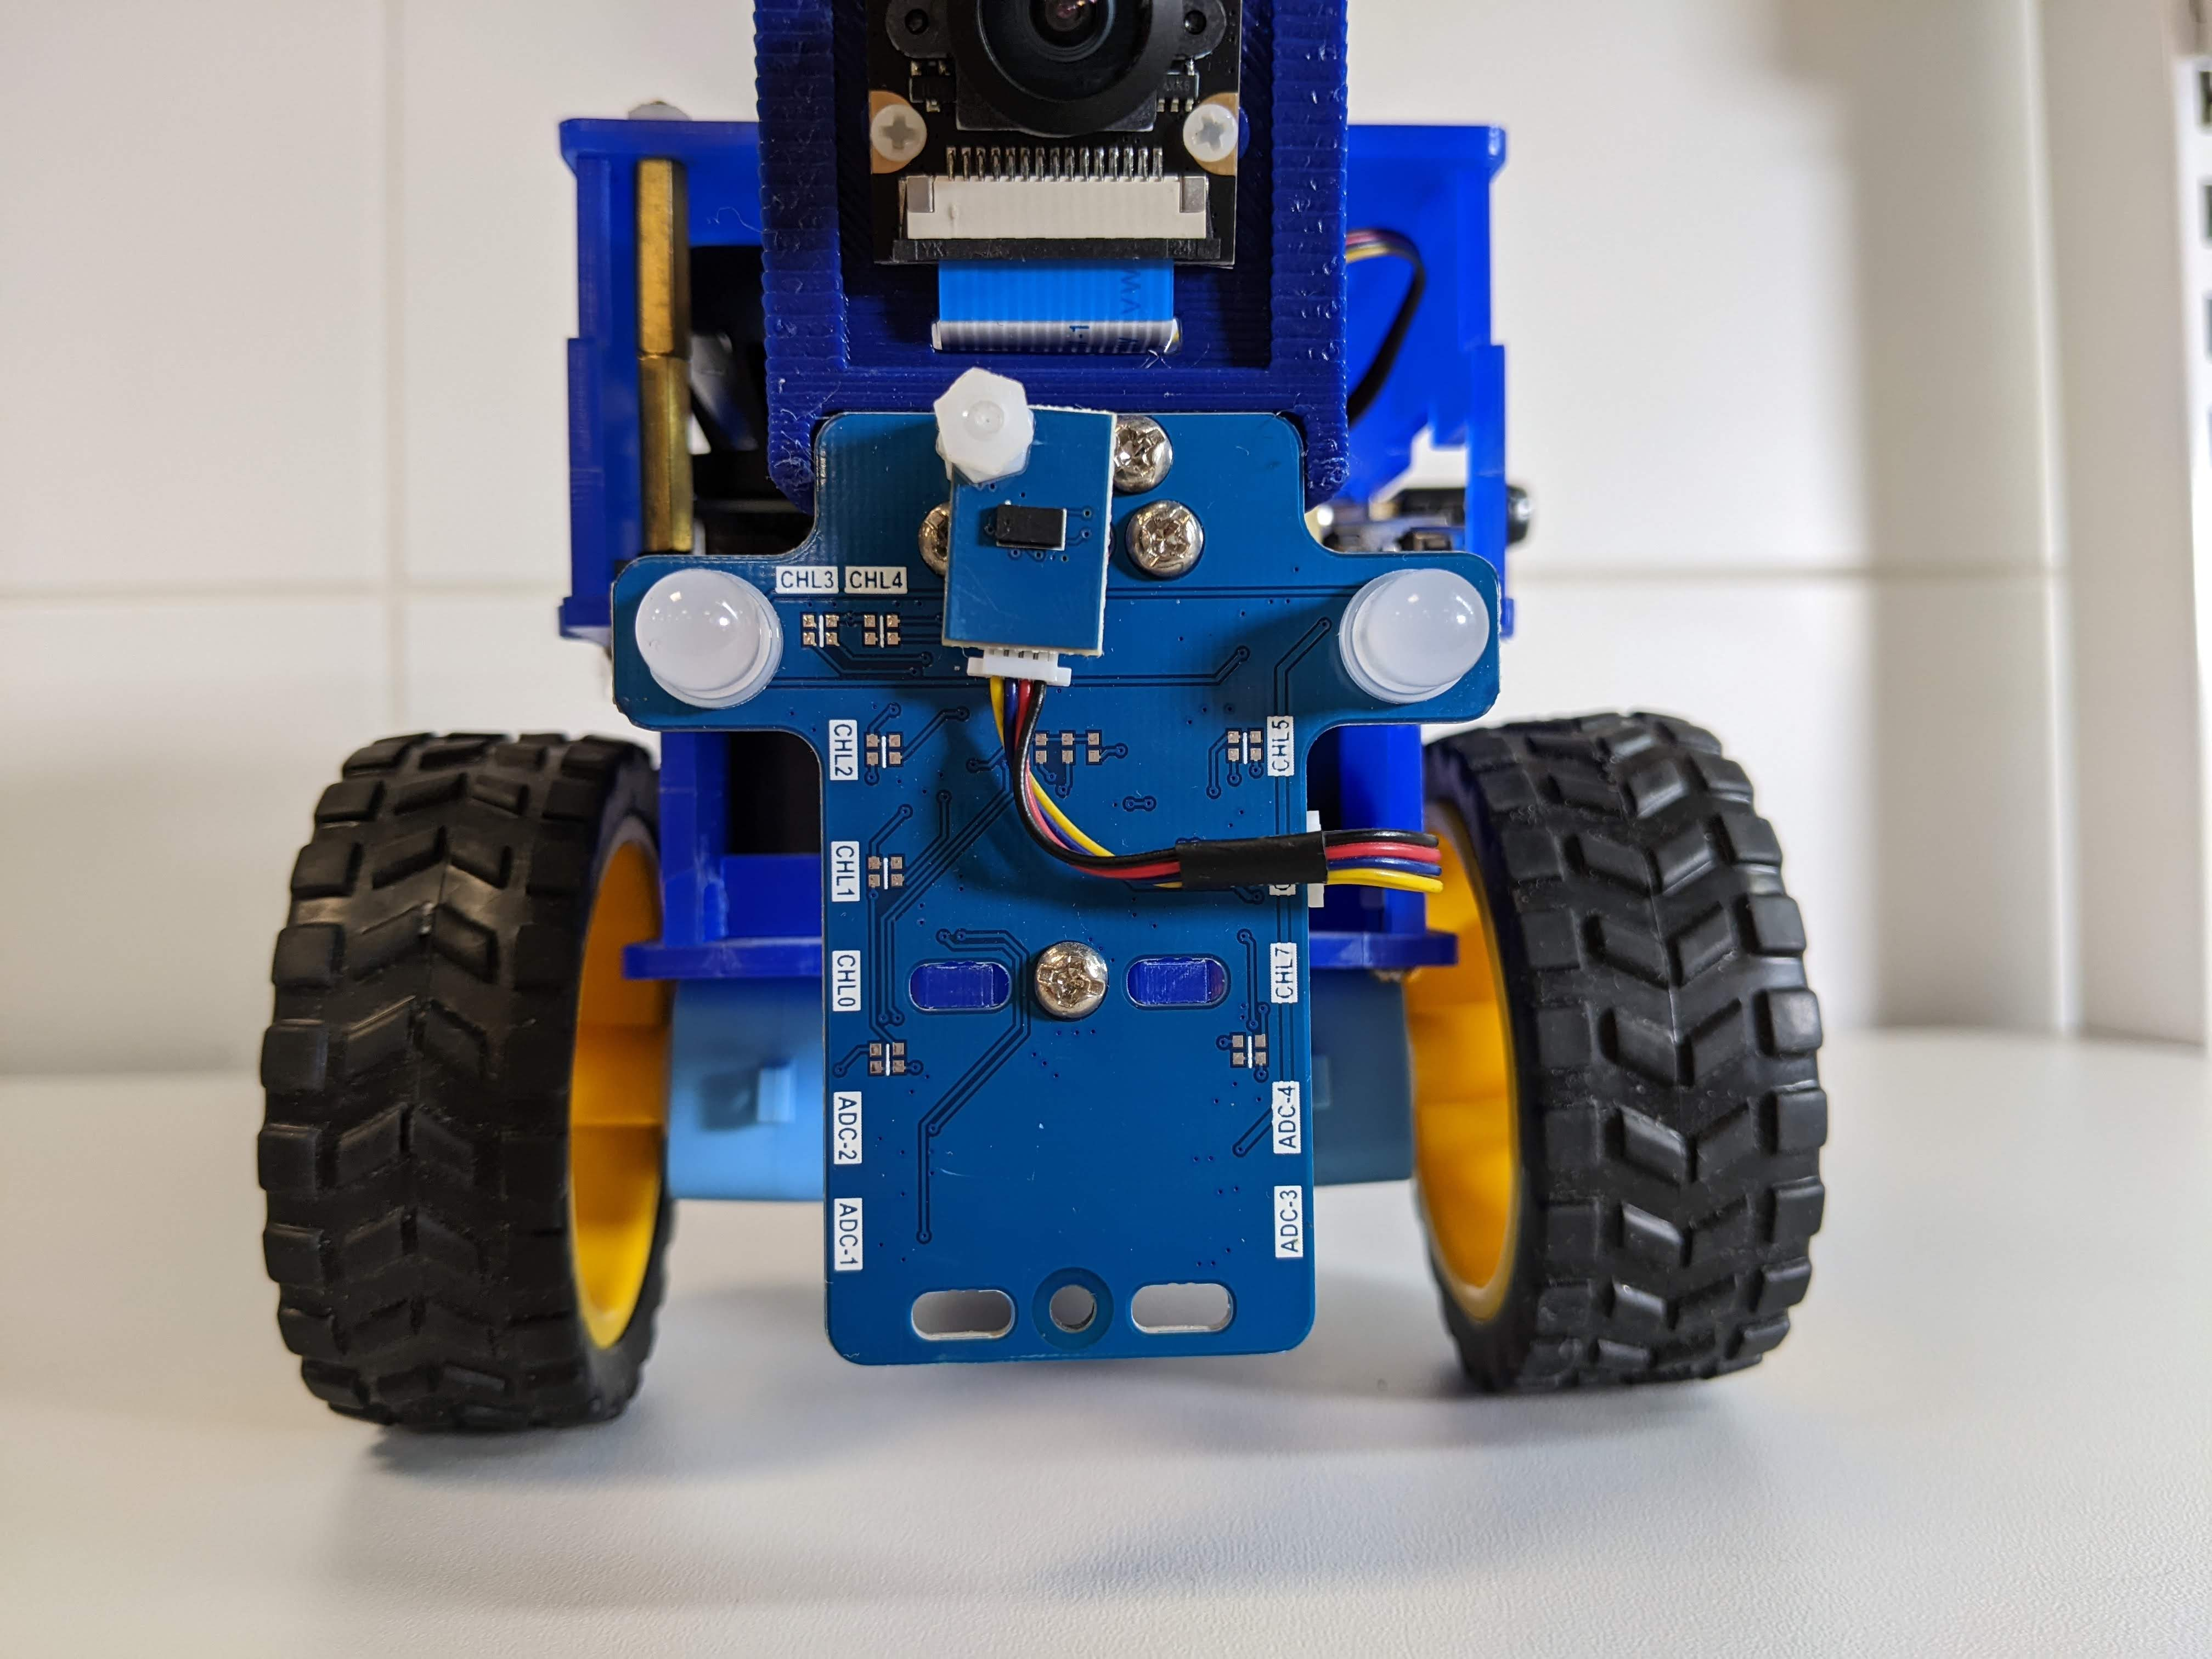
\includegraphics[width=\columnwidth]{PXL_20221207_092836283.jpg}

\subsection{Silniki}
Silnik z przekładnią 120:1, 160 obr/min, moment obrotowy 0,8 kg*cm (0,07 Nm). Urządzenia posiada enkoder kwadraturowy o rozdzielczości 8 impulsów na obrót (po przełożeniu 960 impulsów na obrót).

\href{https://botland.com.pl/silniki-dc-z-przekladnia-i-enkoderami/6287-silnik-z-przekladnia-sj01-120-1-6v-160rpm-enkoder-5904422306793.html}{Botland}, \href{https://www.dfrobot.com/product-1457.html}{DFRobot}

\subsection{Koła}
Koła mają tą wadę, że po pewnym czasie mogą odpaść od wału silnika. Brak jakiejkolwiek możliwości mechanicznego zabezpieczenia przed taką sytuacją. Problem można rozwiązać przy zastosowaniu silników SJ01 na dwa sposoby
\paragraph{Rozwiązanie 1}
Zakup innych typów kół np. \href{https://www.dfrobot.com/product-652.html}{SKU:FIT0199-B} (wymagany dodatkowo  adaptera który nie jest już produkowany \href{https://www.dfrobot.com/product-645.html}{SKU:FIT0198}) lub \href{https://www.dfrobot.com/product-1535.html}{SKU:FIT0500} (większa średnica kół). Można również zakupić koła z firmy Botland \href{https://botland.com.pl/kola-z-oponami/12463-kolo-65x15-mm-biale-5903351248143.html}{DNG-12463}, \href{https://botland.com.pl/kola-z-oponami/13946-kolo-z-opona-65x13mm-biale-5903351248174.html}{DNG-13946}.

\paragraph{Rozwiązanie 2}
Wywiercenie otworów w standardowych kołach (SKU:FIT0003) i przykręcenie ich śruba do wału silnika

\section{Software}
\begin{itemize}
	\item nieaktualna dokumentacja z błędami
\end{itemize}

%
\textcolor{red}{
Ipsum lorem}

\section{Conclusion}
W podsumowaniu należy stwierdzić, że projekt Duckietown pomimo swoich licznych wad jest wartościowy i można z niego korzystać.

\bibliographystyle{plain}
\bibliography{references}

\end{document}
